\documentclass[11pt,a4paper,notitlepage]{report}
\usepackage[british]{babel} % British hyphenation patterns, etc.
\usepackage{csquotes}
\usepackage[T1]{fontenc}
\usepackage{fontspec}
\usepackage[final]{microtype}
\usepackage[a4paper]{geometry}
\usepackage{listings}
\usepackage{titling}
\usepackage[style=ieee,backend=biber]{biblatex}
\usepackage{fancyvrb} % VerbatimInput
\usepackage{tabularx}
\usepackage{graphicx}
\usepackage{floatrow}
\usepackage{enumitem} % noitemsep
\usepackage{tikz}
\usetikzlibrary{chains,shapes,arrows,positioning,backgrounds}

\newenvironment{changemargin}[2]{%
\begin{list}{}{%
\setlength{\topsep}{0pt}%
\setlength{\leftmargin}{#1}%
\setlength{\rightmargin}{#2}%
\setlength{\listparindent}{\parindent}%
\setlength{\itemindent}{\parindent}%
\setlength{\parsep}{\parskip}%
}%
\item[]}{\end{list}}

\addbibresource{references.bib}

\lstset{basicstyle=\small\ttfamily}

% Titlepage formatting
\pretitle{\begin{center}\Huge\bfseries}
\posttitle{\par\end{center}\vspace{0.5em}}
\preauthor{\begin{center}\Large\ttfamily}
\postauthor{\par\large\supervisor\end{center}}
\predate{\par\large\centering}
\postdate{\par\wordcount\par}


% Magic hackery to automaticly generate the word count
\immediate\write18{texcount \jobname.tex -inc -1 -sum -out=wordcount.txt}
\newcommand\wordcount{\small(\input{wordcount.txt}words, counted by
\ttfamily{texcount})}

\title{Binary Code Translation from Register to Stack based code}
\author{Charles Pigott}
\date{DRAFT \today}
\newcommand\supervisor{Supervisor: Christopher Crispin-Bailey}

\begin{document}

\maketitle

%TC:group abstract 0 0
%TC:group lstlisting 0 0
\begin{abstract}
Transmeta are a US based company, who recently surprised the computer
architecture world by developing a chip which dynamically translates Intel
binary code into machine language instructions for another (highly optimised
RISC) CPU core. In doing so it allows Intel code to execute in real-time without
recompilation, but using a (claimed) much more power efficient processor
architecture.

This project attempts to explore something related to the above experiment,
however the focus will be on translating code into potentially parallel sections
using a technique called microthreading. Choosing a relatively simple register
machine for which compiler, assembler, and simulator (or processor) are readily
available would be a sensible approach. The project will involve writing a
translator algorithm in high level code, but if time allows the translator can
be recoded in low-level code, or at least optimised to be as streamlined as
possible (the speed of translation is a critical factor).
\end{abstract}

\cleardoublepage%

\tableofcontents

\chapter{Introduction}\label{ch:introduction}
\section{Aims}
This project aims to show that by converting code written for a simple
register-based architecture or processor to a stack-based architecture,
performance improvements can be found. This will include an example
implementation of translating code intended for a register-based architecture to
run on a stack-based architecture.

\section{Limitations}
Sourcing physical processors and the toolchains capable of running on both the
register-based and stack-based architectures is difficult, as what exists
already tends to be either years out of date, with only partial support, or does
not exist on both platforms. As such, this project will seek to emulate the
architectures instead.

Since the architectures will be emulated, there are precious few advantages to
continuing to use the architecture's native binary code, so this project will
instead take in some form of the respective architecture's assembly language.

\section{Statement of Ethics}
This project does not have any ethical concerns. As Transmeta have already done
a more advanced version of this project nearly two decades ago with their Crusoe
processor, any implications of the results of this project will be unlikely to
affect any commercial businesses. The software produced by this project will be
released open-source once it is completed under a permissive licence, should
anyone else want to take the project further.

\section{Problem approach}
Initially, relevant literature will be reviewed, focusing on the work done by
Transmeta, but also covering computer architectures, code translation and stack
optimisation (Chapter~\ref{ch:litreview}). The knowledge from this will be used
to make a list of requirements for the implentation of the translation program
(Chapter~\ref{ch:problemanalysis}). The program will then be designed and
implemented, documenting the problems and solutions found along the way
(Chapter~\ref{ch:designimplementation}). Once the implementation is complete, it
will be tested appropriately and results will be recorded and evalulated
(Chapter~\ref{ch:testingresults}). Finally, conclusions will be drawn and
further work discussed (Chapter~\ref{ch:conclusions}).


\chapter{Literature Review}
\section{Brief history of computer architectures}
With the exception of Babbage's Analytical Engine, probably the earliest
computer architecture formerly described is that of the EDVAC (Electronic
Discrete Variable Automatic Computer), in 1945 by John von~Neumann in his
incomplete `First Draft of a Report on the EDVAC'. In it, von~Neumann described
a computer which is subdivided into six separate parts - Central Arithmetic
(CA); Central Control (CC); Memory; Input; Output and External Memory (at the
time, this was intended to be something like punched tape). These components
were described using the human nervous sytem as an analogy, with the CA, CC \&
Memory acting as associative (linking) neurons, the Input \& Output acting as
sensory \& motor neurons respectively.
Von~Neumann also wanted to keep the computer as simple as possible, so suggested
that arithmetic operations (such as add and multiply) should not be overlapped,
and performed only one digit at a time. He also noted that external input/output
should first be placed into memory, rather than directly in/out of the CC or CA.
This approach to laying out the components of a computer stuck, and the
approximate idea is still used in modern processors today.\cite{FirstDraft}

\subsection{Register machines}
In the 1950s, logic gates and switches were largely implemented using the quite
large vacuum tubes and discrete transistors. With technology improving,
integrated circuits were invented, constructing logic components using layers of
metal and oxides on polished silicon. Initially, these were only used to
implement individual logic components for computers, replacing the diodes and
resistors used before, until in 1971, Intel released the 4004 microprocessor.
It was the first commercially available fully self contained microprocessor,
with its circuitry fabricated using the new `silicon gate' technology which is
why it was able to be designed and fabricated as one chip. It's worth noting
that Intel as a company didn't have much faith in this product, opting to
instead focus on its line of memory chips and partnering with a Japanese
electronic calculator firm, Busicom, to help finance the project. Nonetheless,
the 4004 was a huge success with 4004 being produced for 10 solid years and
taking Intel to the giant in the computing world that it is
today.\cite{Aspray1997Intel}

\subsection{Stack machines}
Using stacks as part of computation has been around almost as long as computing
itself, with Zuse's Z4 making use of them for subroutines in
1945.\cite{Speiser2000KZZ} These days stacks in computer architectures and
instruction sets are nearly exclusively limited to stack frames, to give the
ability to do context ``saving'' and ``loading'' with function calls, in favour
of register based computation. However, there is a notable exception - the Java
Virtual Machine (JVM) uses a stack-based bytecode as its underlying programming
language.\cite{Schoeberl2005Design}

Instead of having named registers to store values as part of computations, stack
machines use a stack data structure


stack scheduling


\section{Binary Translation}
ibm binary translation

transputer

\subsection{Transmeta Crusoe}
In 2000, Transmeta published a thing which was interesting\cite{TransmetaCodeMorph}



\chapter{Problem Analysis}\label{ch:problemanalysis}
The program implementation should be broken down into a number of steps. First
will be deciding on the source (register) and target (stack) architectures.  The
first part of the implementation will be to implement emulators for the chosen
architectures.  Some conversion routines for register to stack architectures
will be then implemented. After this, the generated stack code will have
optimisation techniques applied to it. Finally, suitable test programs will be
written.

\section{Requirements}
The following is a codified list of required features for the implementation of
the project:

\begin{itemize}[noitemsep]
  \item Fully functioning emulator for a register machine architecture
  \item Fully functioning emulator for a stack machine architecture
  \item Ability to generate stack code from register code
\end{itemize}

There are also a certain number of desirable features that are medium priority.
If these are not implemented, they will be discussed in the further work section (Section~\ref{sec:furtherwork})

\begin{itemize}[noitemsep]
  \item Peephole optimisations on generated stack code
  \item Koopman-style optimisations on generated stack code
\end{itemize}

There are also a few ``nice-to-have'' features, that are low priority and not
all that important for the project to be deemed a `success'.

\begin{itemize}[noitemsep]
  \item Translation threshold --- like the TransMeta implementation, only
  translate regions of code if they are executed more than a certain number of
  times.
  \item Ability to more easily visualise differences between handwritten and
  generated code, e.g.\ graphs or running side-by-side.
\end{itemize}

\chapter{Design and Implementation}

An early decision to be made was to write emulators for the register \& stack
machines chosen. Toolchains for `obscure' architectures such as the ones likely
to be chosen tend to be rather limited in nature and either out-of-date, broken
or both. Writing emulators for the architectures creates extra programming
work, but means that the choices of programming language and style are much
greater.

It was then decided that to simplify the design, the program would be interpret
assembly source code of the register \& stack architectures instead of running
the compiled binary. Doing it this way is only an abstraction over actually
reading the binaries, and skips out having to compile the source code and then
decode it again. Relatively speaking, it would not be difficult to make a
program that does this but was deemed unnecessary for the core part of this
project, converting a register-based instruction set to a stack-based one.

\section{Register based architecture selection}
z80, picoblaze, dcpu-16 choices.
z80 too complex, downgraded to (subset of) dcpu-16, toy cpu created by Markus
Persson for a game
\section{Stack based architecture selection}
J5. probably.



\chapter{Testing, Results and Evaluation}\label{ch:testingresults}

Due to the emulated nature of the implementation of this project, the only
meaningful metric that can be taken from the results would be comparing
instruction counts between the register program and the unoptimised and
optimised stack programs.

Testing will be done using a series of programs handwritten for the DCPU-16
emulator. They vary between simple test programs (for compiler correctness) and
full benchmarking programs. The test programs were purely for verifying
emulator \& optimiser correctness and will not be discussed in further detail.

\begin{itemize}[noitemsep]
  \item \texttt{simple} --- Single addition test
  \item \texttt{loop} --- Loop test
  \item \texttt{redundant} --- Program with deliberately redundant register
  usage
    \vspace{2ex}
  \item \texttt{bsort} --- Bubble sort benchmark. Sorts 32 integers and prints
  the result
  \item \texttt{fib20} --- Calculates and prints the first 20 fibonacci numbers
  \item \texttt{primes} --- Uses a prime sieve to get all the prime numbers up
  to 100
  \item \texttt{tri100} --- Outputs the first 100 triangle numbers, using the
    addition formula
\end{itemize}

\section{Results}

\begin{table}
  \begin{tabular}{r r r r}
                    &   Base & Peephole & Koopman \\ \toprule
    \texttt{bsort}  &  24024 &    22343 &   22233 \\ \midrule
    \texttt{fib20}  &    665 &      608 &     606 \\ \midrule
    \texttt{primes} &   6717 &     6619 &    6619 \\ \midrule
    \texttt{tri100} & 111381 &   106332 &  106332 \\ \midrule
  \end{tabular}
  \caption{No.\ of instructions executed}\label{tab:instructions}
\end{table}

\begin{table}
  \begin{tabular}{r r r r}
                    &  Base & Peephole & Koopman \\ \toprule
    \texttt{bsort}  &  7792 &     6703 &    6065 \\ \midrule
    \texttt{fib20}  &   234 &      196 &     175 \\ \midrule
    \texttt{primes} &  1912 &     1912 &    1643 \\ \midrule
    \texttt{tri100} & 35345 &    35345 &   30296 \\
  \end{tabular}
  \caption{No.\ of LOAD/STORE instructions executed}\label{tab:meminstructions}
\end{table}

\pgfplotstableread[col sep=comma,header=false]{%
bsort,24024,22343,22233
fib20,665,608,606
primes,6717,6619,6619
tri100,111381,106332,106332
}\tracedata%

\pgfplotstableread[col sep=comma,header=false]{%
bsort,7792,6703,6065
fib20,234,196,175
primes,1912,1912,1643
tri100,35345,35345,30296
}\tracememdata%

\pgfplotsset{%
  relative series/.style={%
    table/y expr=\thisrow{#1}/\thisrow{1},
    table/meta=#1
  },
  relative graph/.style={%
    width=13cm,
    ymajorgrids=true,
    major x tick style = transparent,
    major y tick style = transparent,
    scaled y ticks = false,
    ybar=0pt,
    ymin=0.5,
    bar width=0.75cm,
    enlarge x limits=0.2,
    symbolic x coords={bsort,fib20,primes,tri100},
    xtick=data,
    legend cell align=left,
    legend style={%
      at={(1,0)},
      anchor=south west,
      column sep=1ex
    }
  }
}

\begin{figure}
  \begin{tikzpicture}
    \begin{axis}[relative graph]
      \addplot table [relative series=1] {\tracedata};
      \addplot table [relative series=2] {\tracedata};
      \addplot table [relative series=3] {\tracedata};
      \legend{Base,Peephole,Koopman}
    \end{axis}
  \end{tikzpicture}
  \caption{Relative no.\ of instructions executed}\label{fig:relativeinstructions}
\end{figure}

\begin{figure}
  \begin{tikzpicture}
    \begin{axis}[relative graph]
      \addplot table [relative series=1] {\tracememdata};
      \addplot table [relative series=2] {\tracememdata};
      \addplot table [relative series=3] {\tracememdata};
      \legend{Base,Peephole,Koopman}
    \end{axis}
  \end{tikzpicture}
  \caption{Relative no.\ of LOAD/STORE instructions executed}\label{fig:relativememinstructions}
\end{figure}

Tables~\ref{tab:instructions} \&~\ref{tab:meminstructions} represent the number
of instructions executed for a complete run of the benchmark programs, and the
number of LOAD/STORE operations for each of them for the same run, respectively.
Figures~\ref{fig:relativeinstructions} \&~\ref{fig:relativememinstructions}
graph the relative decrease in the number of instructions executed for each
optimisation level, where no optimisations is the base level at one.

\begin{table}
\begin{tabular}{l l r r r r}
  Program & Block & Register & Stack & Peephole & Koopman \\ \toprule
  \multirow{6}{*}{\texttt{bsort}}  & & 34 & 103 & 102 & 102 \\
  & \texttt{LOOP}                    &  2 &   9 &   8 &   8 \\
  & \texttt{LOOP2}                   &  5 &  25 &  24 &  24 \\
  & \texttt{SWAP}                    &  3 &  24 &  24 &  23 \\
  & \texttt{POST}                    &  6 &  27 &  25 &  25 \\
  & \texttt{RESL}                    &  4 &  22 &  21 &  21 \\ \midrule
  \multirow{2}{*}{\texttt{fib20}}  & &  6 &  34 &  32 &  32 \\
  & \texttt{LOOP}                    &  7 &  20 &  20 &  18 \\ \midrule
  \multirow{5}{*}{\texttt{primes}} & &  2 &   6 &   6 &   6 \\
  & \texttt{LOOP}                    &  2 &  12 &  12 &  12 \\
  & \texttt{SCANNED}                 &  4 &  17 &  16 &  16 \\
  & \texttt{SCAN}                    &  3 &  17 &  17 &  17 \\
  & \texttt{LOOP2}                   &  4 &  24 &  24 &  24 \\ \midrule
  \multirow{5}{*}{\texttt{tri100}} & &  2 &   6 &   6 &   6 \\
  & \texttt{LOOP}                    &  2 &   6 &   6 &   6 \\
  & \texttt{LOOP2}                   &  4 &  20 &  19 &  19 \\
  & \texttt{BREAK}                   &  4 &  23 &  22 &  22 \\
\end{tabular}
\caption{Instruction execution counts per block}\label{tab:instructionperblock}
\end{table}

\pgfplotstableread[col sep=comma]{%
Register,Stack,Peephole,Koopman
%34,103,102,102
2,9,8,8
5,25,24,24
3,24,24,23
6,27,25,25
4,22,21,21
6,34,32,32
7,20,20,18
2,6,6,6
2,12,12,12
4,17,16,16
3,17,17,17
4,24,24,24
2,6,6,6
2,6,6,6
4,20,19,19
4,23,22,22
}\blockdata%

\begin{figure}
  \begin{tikzpicture}
    \begin{axis}[
        xlabel=No.\ of register instructions,
        ylabel=No.\ of stack instructions,
        legend cell align=left,
        legend style={%
          at={(1,0)},
          anchor=south west,
          column sep=1ex
        }
    ]
      \addplot [only marks,mark=x,blue] table [y=Stack] {\blockdata};
      \addplot [thick,blue] table [y={create col/linear regression={y=Stack}}] {\blockdata};
      \addlegendentry{Base}
      \addplot [only marks,mark=x,red] table [y=Peephole] {\blockdata};
      \addplot [thick,red] table [y={create col/linear regression={y=Peephole}}] {\blockdata};
      \addlegendentry{Peephole}
      \addplot [only marks,mark=x,brown] table [y=Koopman] {\blockdata};
      \addplot [thick,brown] table [y={create col/linear regression={y=Koopman}}] {\blockdata};
      \addlegendentry{Koopman}
      \legend{Base,,Peephole,,Koopman}
    \end{axis}
  \end{tikzpicture}
  \caption{Graph of register blocks to stack equivalents}\label{fig:instructionperblock}
\end{figure}

Table~\ref{tab:instructionperblock} lists the number of stack instructions
produced per block of register code, for different optimisation levels. The
`empty' block row represents the initial block of the program, with no label. It
is graphed in Figure~\ref{fig:instructionperblock}. Notably for the graph, the
initialisation block for bsort is omitted as it is considerably larger than
anything else and considered anomalous.


\section{Evaluation}\label{sec:testingevaluation}
The basic results (Seen in Table~\ref{tab:instructions} and
Figure~\ref{fig:relativeinstructions}) show some interesting results, showing
that Peephole optimisation does the bulk of the the overall executed instruction
count reduction and that Koopman-style stack scheduling has very little effect.

However, looking at the number of memory reads \& writes (with \lstinline{LOAD}
\& \lstinline{STORE} respectively) in Table~\ref{tab:meminstructions} (and
visualised in Figure~\ref{fig:relativememinstructions}) shows a different
result, with stack scheduling doing as much reduction as peephole optimisation
if not more, particularly in the case of the \texttt{primes} \& \texttt{tri100}
programs which have no instruction decrease with stack scheduling, but a
significant decrease in memory usage.

While the optimisation results are good (30\% reduction in memory usage is
quite substantial), it is not the same as promised by Koopman in his original
paper. Koopman claimed to be able to remove 90--100\% of redundant local
variable accesses. The results here are not quite the same measurement, but it
is hard to believe that they are the same number which is difficult to
programatically calculate --- Koopman did it by studying the program's output by
hand. It is possible that the results are so different due to the programs used
--- `tight loops' that don't make much use of variable accesses won't have as
many opportunities for stack scheduling as others.

\subsection{Completion of requirements}
All key features of the project were completed, but only one of the desirable
features was able to be partially implemented, largely due to time constraints.

Both register and stack emulators were implemented and able to accurately
emulate their respective assembly languages. Stack code was able to be generated
from register code which was correct and free of other side effects. Both
peephole optimisations and stack-scheduling were implemented as optional
features in the conversion routines that can be enabled at will with command
flags (similar to optimise flags in C++ compilers).



\subsection{Program correctness}
No significant automated testing of the implementation has been done. Instead
the program's output was verified ``by eye'' and for the test run the multiple
executions were compared against each other, to ensure consistent results.

\subsection{Code quality}
The code itself is relatively extensible for future work. It is published as
open-source software at \texttt{github.com/LordAro/reg2stack} enabling any
future work to be able to be built on top of this software. The peephole
optimsation implementation allows for easy additions --- just add the relevant
function and add the function name to the list of existing functions.

Documentation of the code could definitely be improved. While complicated code
generally has comments explaining exactly why it does what it does, it's by no
means complete and could certainly be expanded. Many functions are also missing
`doccoments', which generally take the form of comments above the function
definition which can then be parsed by some external tool to generate more
formal documentation. If this were expanded it would be really helpful to future
work done on the program.

\chapter{Conclusions}\label{ch:conclusions}
This project set out to show that it was possible to get performance
improvements out of stack machine code that was generated from code intended for
a register-based architecture. Ultimately, the results for this project resulted
in around a 10\% decrease in raw stack instruction count and up to 25\% decrease
in number of memory accesses. More significant results were seen with conversion
block caching, seeing an up to 60\% decrease in relative program cost based on
an estimated memory model. The implementation was also designed in such a way
that allows for further optimisations and improvements to be made to the
project and the software was released on GitHub to facilitate this.

All requirements to the project as defined in Problem Analysis
(Chapter~\ref{ch:problemanalysis}) were evaluated
(Section~\ref{sec:testingevaluation}) and it was found that all key requirements
were completed and but there was only partial completion of one of the optional
requirements. Both register architectures had ``feature complete'' emulators
that were able to parse and run their respective assembly code. Stack code is
able to be generated from each register instruction, with the ability to
translate whole programs, one block at a time. Through the use of commandline
flags, two different optimisation levels can be used --- peephole \&
stack-scheduling --- which reduce both instruction count and the number of
memory accesses compared to the unoptimised output.  Finally each converted
block was able to be cached, saving effort on converting it multiple times when
looped over.

The results of the tests vary depending on the program, but they generally
result around a 10\% decrease in raw stack instruction count and up to 25\%
decrease in number of memory accesses, importantly showing that stack machines
are not inherently less efficient at dealing with data accesses than register
machines. More significant and varied results were seen with conversion block
caching, with results varying from no improvement at all to up to 60\% decrease
in relative program cost based on the estimated memory model.

In conclusion, this project was able to show that there were several
improvements to be found in stack code generated from code intended for a
register machine.

\section{Further work}\label{sec:furtherwork}
There are several further steps that could be applied to this project.

First and foremost would be to implement further optimisations, such as the
inter-block algorithm by Bailey and the refinements done by Shannon show great
potential for further improvements especially with the tight loops of the
programs tested in this project.

There's also further scope for improving the instruction block caching system.
Other than improving how blocks are divided up, making use of Transmeta's
`translation threshold' method could prove more effective for reducing the
relative cost of running a program. Further work could also be put into using a
more accurate memory model, as the results of the program cost
(Figure~\ref{fig:progcost}) from the one used in this project are only drawn
from an approximation taken from a flat memory model and an estimated cost for
translation.

Other options would be to more properly prove that the implementation of the
emulators, and the conversion routines is correct. Formal methods to
mathematically prove correctness could even be used if so inclined. This could
be taken further to automatically generate test programs that try to break the
conversion or the emulators, generally referred to as ``fuzz testing''

An ambitious goal would be to implement the conversion and optimisation routines
in the target stack architecture. This would mean that the the conversion could
be implemented natively on a processor capable of running the stack program.
Such a program would be very complicated so a stack language capable of
high-level features such as functions would be necessary to make this goal
feasible.


\addcontentsline{toc}{chapter}{Bibliography}
\printbibliography%
\clearpage

%TC:ignore
\appendix
\chapter{DCPU-16 Specification}\label{ch:dcpuspec}
\VerbatimInput[fontsize=\footnotesize]{dcpu16.txt}

\chapter{Simplified J5 Instruction Sheet}\label{ch:j5spec}
Transcribed from 2013 DACS Exam paper
\subsubsection{Arithmetic \& Logical}
\begingroup
\ttfamily
\begin{tabularx}{0.95\textwidth}{l X}
  ADD & Add Top \& Next on stack together   (3,2) -> (5) \\
  SUB & Subtract Top from Next on stack   (2,8) -> (6) \\
  INC & Increment Top of stack \\
  DEC & Decrement Top of stack \\
  AND/OR/NOT/XOR & Combine Top \& Next in in logical operation \\
  SHR & Shift Top of stack 1 bit to right \\
  SHL & Shift Top of stack 1 bit to left \\
\end{tabularx}
\endgroup

\subsubsection{Comparative}
\begingroup
\ttfamily
\begin{tabularx}{0.95\textwidth}{l X}
  TGT & Test Top greater than Next, set Zero flag to true or false* \\
  TLT & Test Top less than Next, set Zero flag to true or false* \\
  TEQ & Test Top equal to Next, set Zero flag to true or false* \\
  TSZ & Test Top set to zero, set Zero flag to true or false* \\
\end{tabularx}
\endgroup

\hfill*Note these do not destroy Top and Next when they are operated.

\subsubsection{Other instructions}
\begingroup
\ttfamily
\begin{tabularx}{0.95\textwidth}{l >{\raggedright\arraybackslash}X}
  SSET n & Place an operand n on the stack \\
  SET nn & Place an operand nn on the stack \\
  LOAD & Take address from Top of stack, access location, put result on stack \\
  STORE & Take Top as address, and Next as data, then write data to the address
  \\
  BRANCH nn & Unconditional relative branch of +/- nn bits \\
  BRZERO nn & Conditional branch (taken if Zero Flag set) \\
  IBRANCH & Indirect branch PC <= M[TOS] \\
  CALL nn & Call to address nn \\
  RETURN & Return from call \\
  STOP & Causes Execution to halt \\
\end{tabularx}
\endgroup

\subsubsection{Stack manipulations}
\begingroup
\ttfamily
\begin{tabularx}{\textwidth}{l >{\raggedright\arraybackslash}X r}
  DROP    & Drop an item from the Top of the stack   & \\
  DUP     & Duplicate Top of stack                   & (X,Y) -> (X,X,Y)     \\
  SWAP    & Swap Top and Next                        & (X,Y) -> (Y,X)       \\
  RSD3    & Rotate stack down three                  & (X,Y,Z) -> (Z,X,Y)   \\
  RSU3    & Rotate stack up three                    & (X,Y,Z) -> (Y,Z,X)   \\
  TUCK2   & Tuck copy of Top under 2nd item          & (X,Y,Z) -> (X,Y,X,Z) \\
  TUCK3   & Tuck copy of Top under 3rd item          & (X,Y,Z) -> (X,Y,Z,X) \\
  COPY3   & Copy 3rd stack item to Top of stack      & \\
  PUSH rr & Push register (F,LBR,GBR,VBA) onto stack & \\
  POP rr  & Pop register (F,LBR,GBR,VBA) from stack  & \\
\end{tabularx}
\endgroup

\subsubsection{Registers}
The J5 has the usual stack registers, Top, Next, 3rd, etc, and also has Local
Base Register (\textbf{LBR}), Global Base Register (\textbf{GBR}), Vector Base
Address (\textbf{VBA}), and an F register containing the flags shown below.

\vspace{10mm}

\noindent\begin{minipage}[b]{0.5\linewidth}
  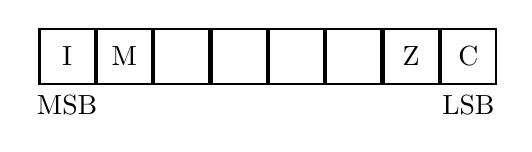
\begin{tikzpicture}
    \tikzstyle{every path}=[thick]
    \edef\turingtapesize{0.7cm}
    \tikzstyle{tmtape}=[draw,minimum size=\turingtapesize]

    \begin{scope}[start chain=1 going right,node distance=0mm]
      \node[on chain=1,tmtape,label=below:MSB] {I};
      \node[on chain=1,tmtape]                 {M};
      \node[on chain=1,tmtape]                 {};
      \node[on chain=1,tmtape]                 {};
      \node[on chain=1,tmtape]                 {};
      \node[on chain=1,tmtape]                 {};
      \node[on chain=1,tmtape]                 {Z};
      \node[on chain=1,tmtape,label=below:LSB] {C};
    \end{scope}
  \end{tikzpicture}
\end{minipage}%
\noindent\begin{minipage}[b]{0.5\linewidth}
  \textbf{C}-Carry Flag\@ \textbf{Z}-Zero Flag\\
  \textbf{I}-Interrupt (1=Enable, 0=Disable)\\
  \textbf{M}-Interrupt Mode (1=Vector, 0=Opcode)
\end{minipage}

\chapter{Benchmark programs}\label{ch:benchmarkprograms}
\begin{lstlisting}[caption={bsort.reg}]
; initial "input"
SET [0x3000], 6221
SET [0x3001], 16181
SET [0x3002], 29598
SET [0x3003], 10115
SET [0x3004], 18953
SET [0x3005], 44337
SET [0x3006], 12629
SET [0x3007], 7527
SET [0x3008], 56169
SET [0x3009], 44334
SET [0x300a], 2290
SET [0x300b], 38260
SET [0x300c], 62627
SET [0x300d], 9740
SET [0x300e], 40652
SET [0x300f], 58444
SET [0x3010], 21421
SET [0x3011], 45306
SET [0x3012], 38396
SET [0x3013], 25410
SET [0x3014], 31580
SET [0x3015], 17208
SET [0x3016], 27939
SET [0x3017], 59297
SET [0x3018], 55094
SET [0x3019], 45095
SET [0x301a], 55388
SET [0x301b], 30943
SET [0x301c], 33757
SET [0x301d], 48729
SET [0x301e], 42
SET [0x301f], 29832

SET [0x2fff], 32 ; length

; sort
SET J, [0x2fff]
:LOOP SUB J, 1
	SET I, 0
:LOOP2 SET A, [0x3000+I]
	SET B, [0x3000+J]
	IFG A, B ; compare
		SET PC, SWAP
	SET PC, POST
:SWAP SET C, [0x3000+I]
	SET [0x3000+I], [0x3000+J]
	SET [0x3000+J], C
:POST ADD I, 1
	IFG J, I
		SET PC, LOOP2
	IFN J, 0
		SET PC, LOOP

; output result
SET I, 0
:RESL OUT [0x3000+I]
	ADD I, 1
	IFN I, [0x2fff]
		SET PC, RESL
\end{lstlisting}

\begin{lstlisting}[caption={fib20.reg}]
SET [0x2000], 20 ; limit

SET A, 0 ; F(0)
SET B, 1 ; F(1)

OUT A
OUT B

SET I, 1
:LOOP SET C, A
	SET A, B
	ADD B, C
	OUT B
	ADD I, 1
	IFN I, [0x2000]
		SET PC, LOOP
\end{lstlisting}

\noindent\begin{minipage}{\linewidth}
\begin{lstlisting}[caption={primes.reg}]
SET I, 100 ; limit
SET A, 2
:LOOP IFE [A+3000], 0
	SET PC, SCAN
:SCANNED ADD A, 1
IFG A, I
    SET PC, PC ; we're done
SET PC, LOOP

:SCAN IFL A, I
	OUT A
SET B, A
:LOOP2 SET [B+3000], 1
ADD B, A
IFL B, I
	SET PC, LOOP2
SET PC, SCANNED
\end{lstlisting}
\end{minipage}

\begin{lstlisting}[caption={tri100.reg}]
SET C, 100 ; limit
SET I, 1
:LOOP SET J, 0
SET B, 0
:LOOP2 ADD J, 1
ADD B, J
IFL J, I
  SET PC, LOOP2
:BREAK OUT B
ADD I, 1
IFL I, C
  SET PC, LOOP
\end{lstlisting}

%TC:endignore
\end{document}
